\section{Results}
The results section is divided into three subsections, each corresponding to the individual research questions as described in the \textit{introduction} section. (R1) Relateing to activity of political parties on the platform, (R2) relating to topics from election manifestos and voting guides, and (R3) relating to a network analysis of instances and servers of political parties on the network. Each with accompanying descriptions of the methods performed and graphs to further understand the data and the result of the analysis.

A clear increase in general activity surrounding the Dutch elections on the platform is found.
When querying toots with general terms on Dutch elections, for example “verkiezingen”, “ducth elections”, or “tweede kamer”, the results have very clearly spiked in the last period, as shown in figure \ref{fig:electionstotal}. A total of 18,230 toots were retrieved, which included these election related terms, of which around 16,000 are in the last two years.
Therefore, Mastodon has been more widely adopted for the most recent election year, 2023, as opposed to previous elections, 2017 and 2021, which showed almost no activity on these general queries.

\begin{figure}[ht]
  \centering
  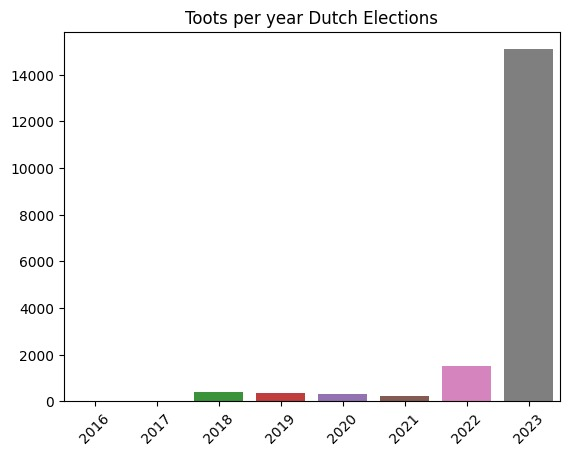
\includegraphics[width=3.25in]{media/dutch-elections-mastodon.jpeg}
  \caption{Bar chart of query word results, using general terms surrounding Dutch elections}
  \label{fig:electionstotal}
\end{figure}

\subsection{Activity of Political Parties (R1)}

\begin{figure*}[ht]
  \centering
  \begin{subfigure}[h]{.49\linewidth}
    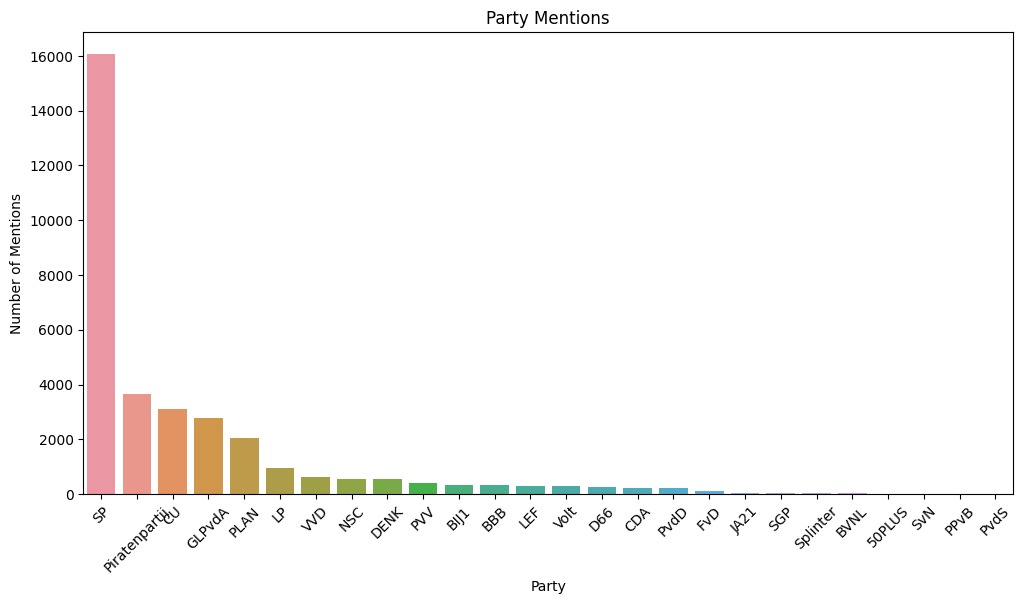
\includegraphics[width=\textwidth]{media/party-mentions.jpeg}
    \captionsetup{justification=centering}
    \caption{Bar chart showing individual political party mentions}
    \label{fig:partymentions}
  \end{subfigure}
  \begin{subfigure}[h]{.49\linewidth}
      \captionsetup{justification=centering}
      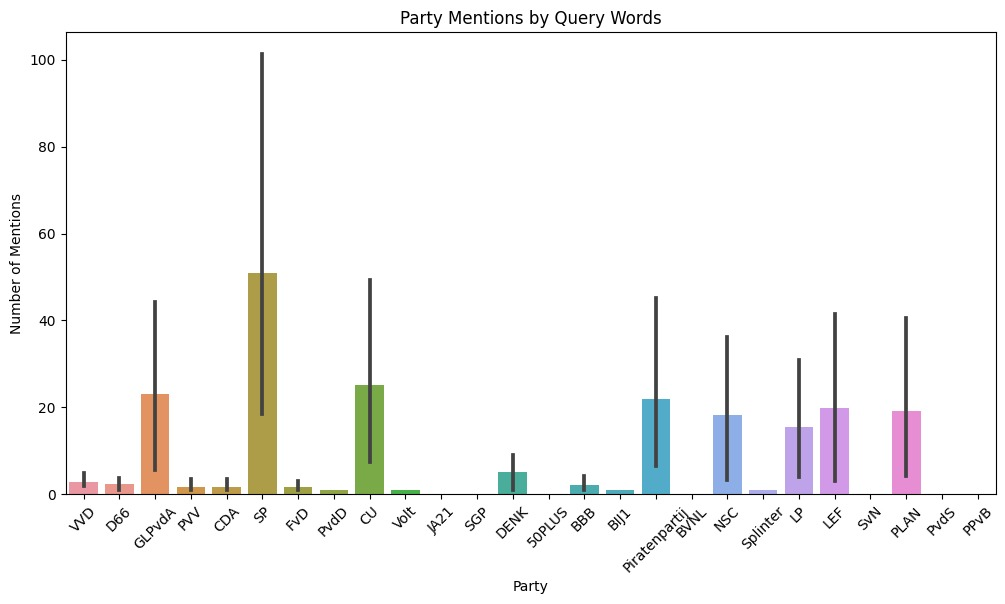
\includegraphics[width=\textwidth]{media/party-mentions-query-words.jpeg}
      \caption{Candlestick chart showing parties being mentioned based on topical query words. The wick represents the spread of unique topics}
      \label{fig:partycandle}
  \end{subfigure}
  \caption{Graphs visualizing party activity based on party name mentions and query words based on topics}
  \label{fig:results}
\end{figure*}

\textbf{Finding M1:} \textit{Out of all parties x parties are present on Mastodon and have instances.}

\subsection{Election-related topics and query words (R2)}

\begin{figure}[ht]
  \centering
  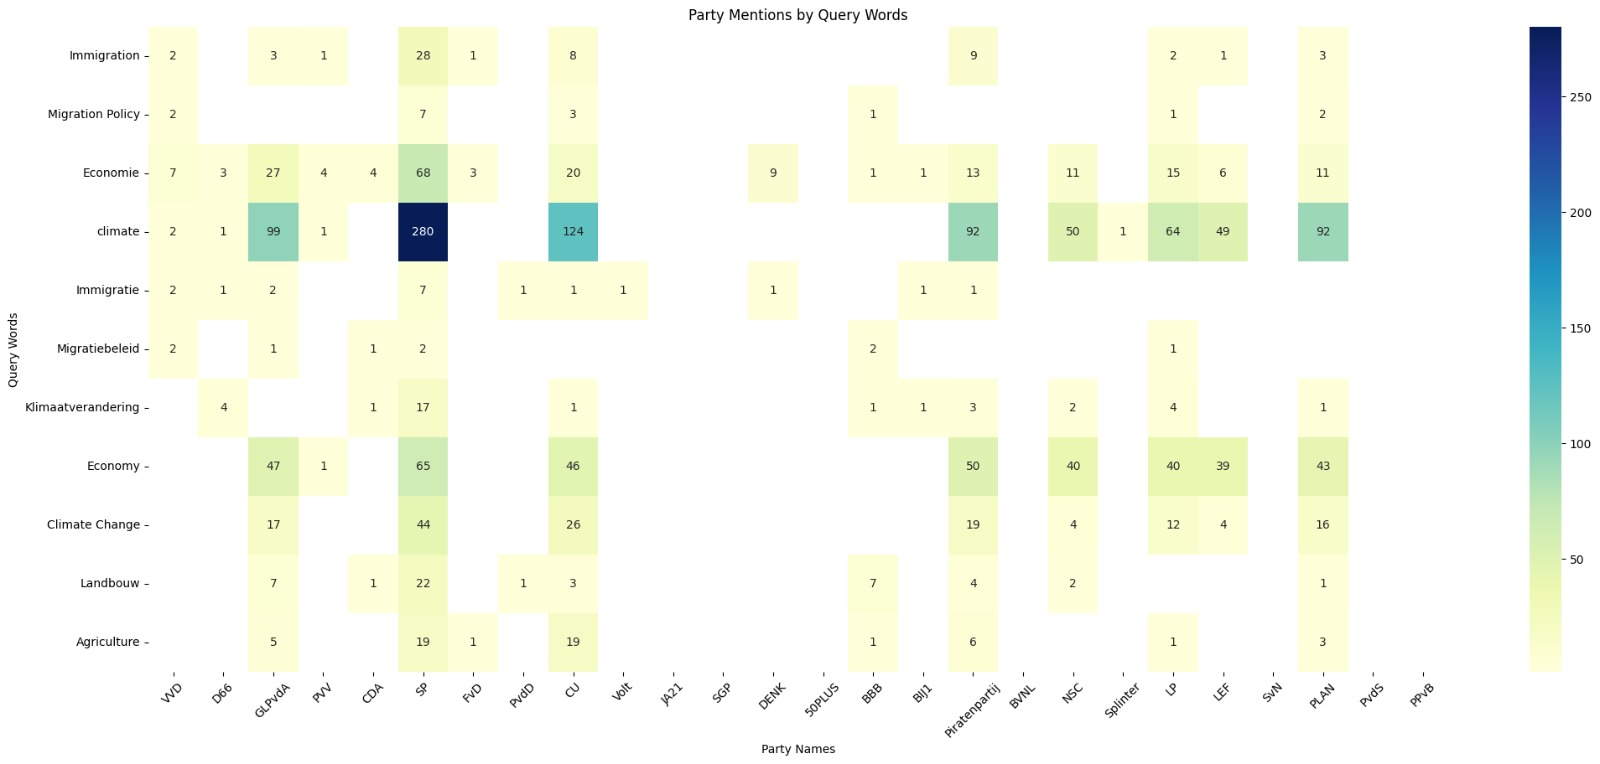
\includegraphics[width=\linewidth]{media/party-mentions-topics.jpeg}
  \caption{Party mentions related to topics}
  \label{fig:topic}
\end{figure}


\textbf{Finding M2:} \textit{Out of all parties, x parties are present on Mastodon and have instances.}

\subsection{Analysis of Party accounts and servers (R3)}
To han

\begin{figure}[ht]
  \centering
  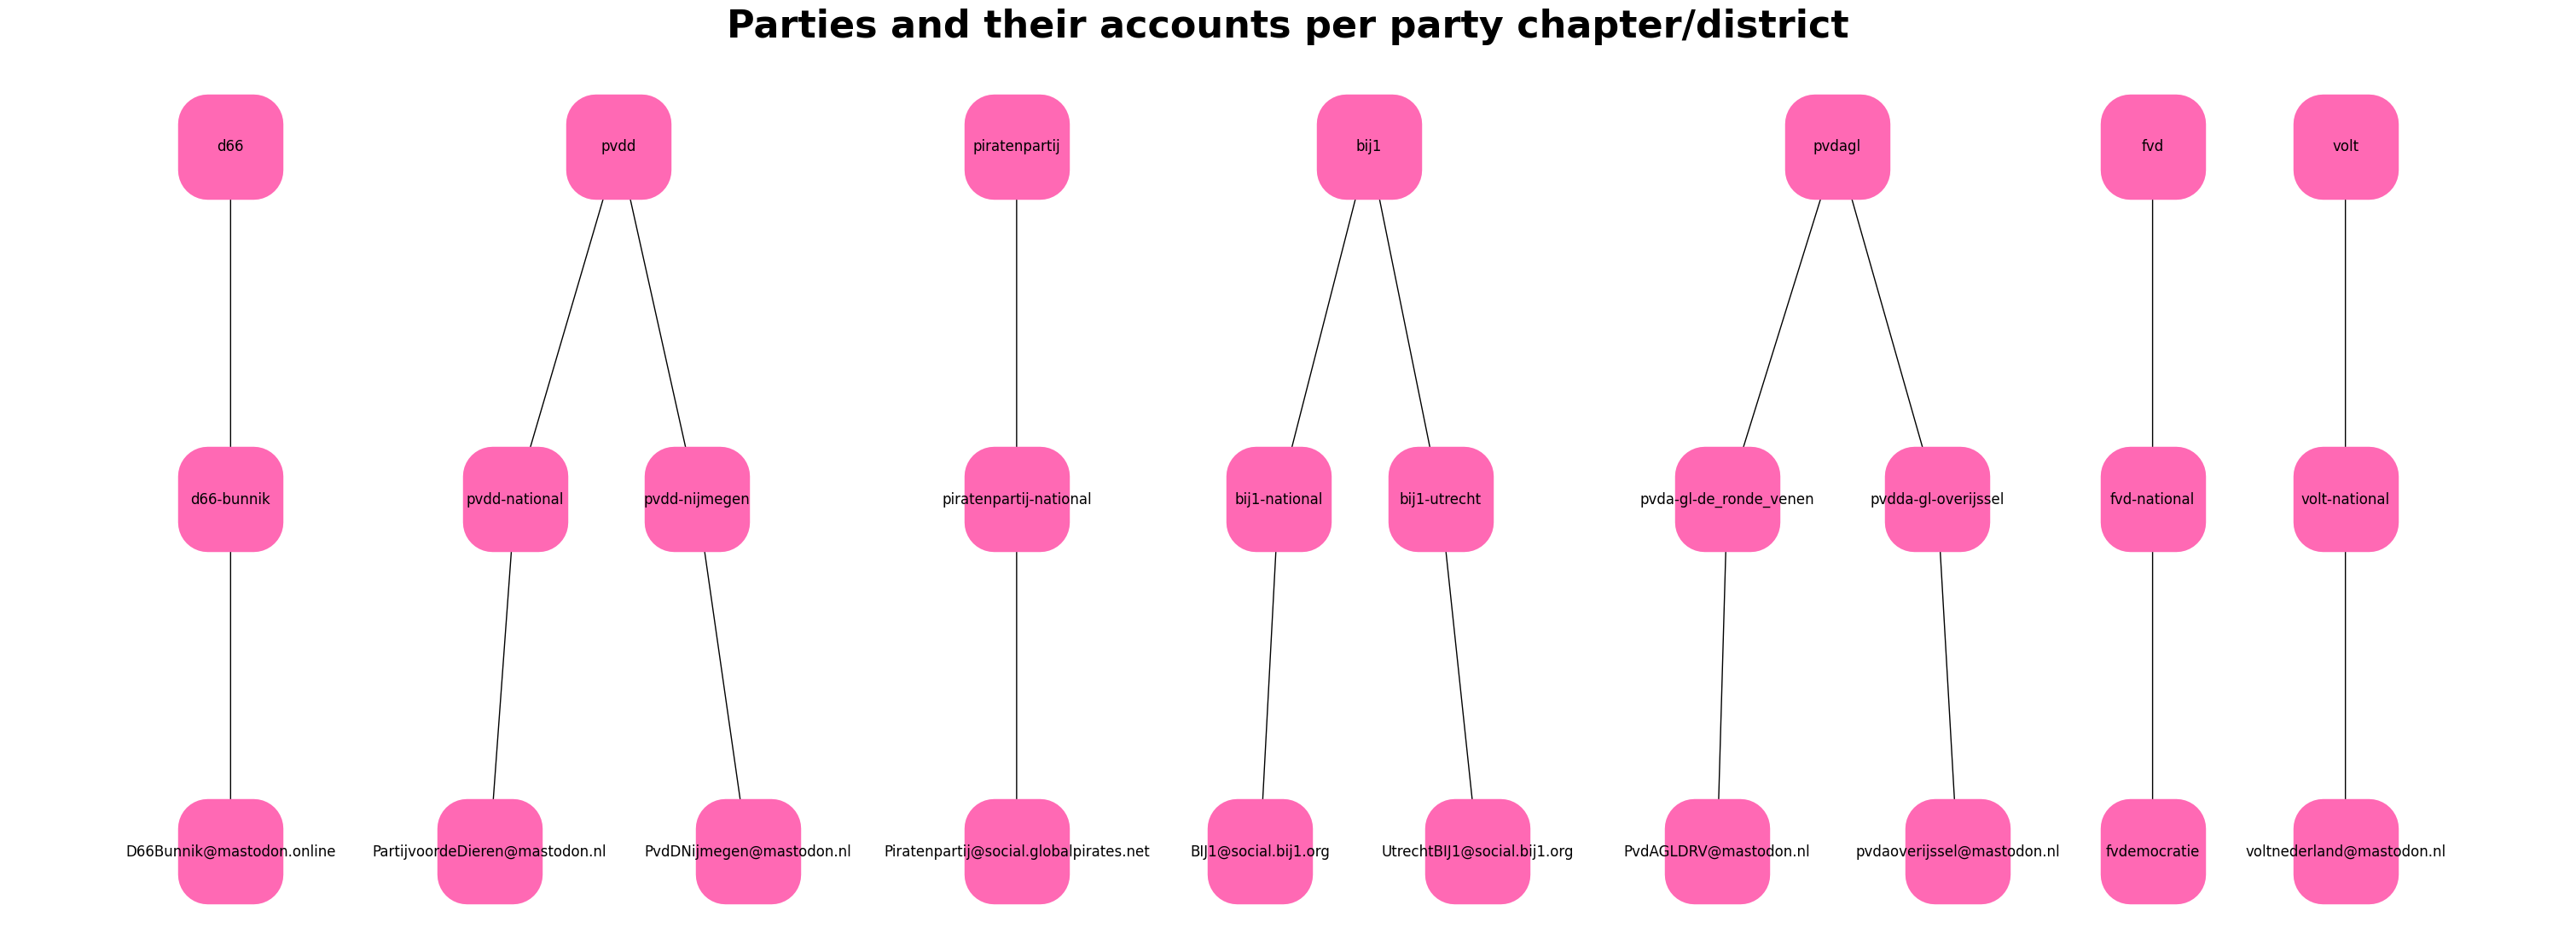
\includegraphics[width=\linewidth]{media/chapter.png}
  \caption{Tree of party accounts, branching from their district}
  \label{fig:partynetwork}
\end{figure}

\begin{figure}[ht]
  \centering
  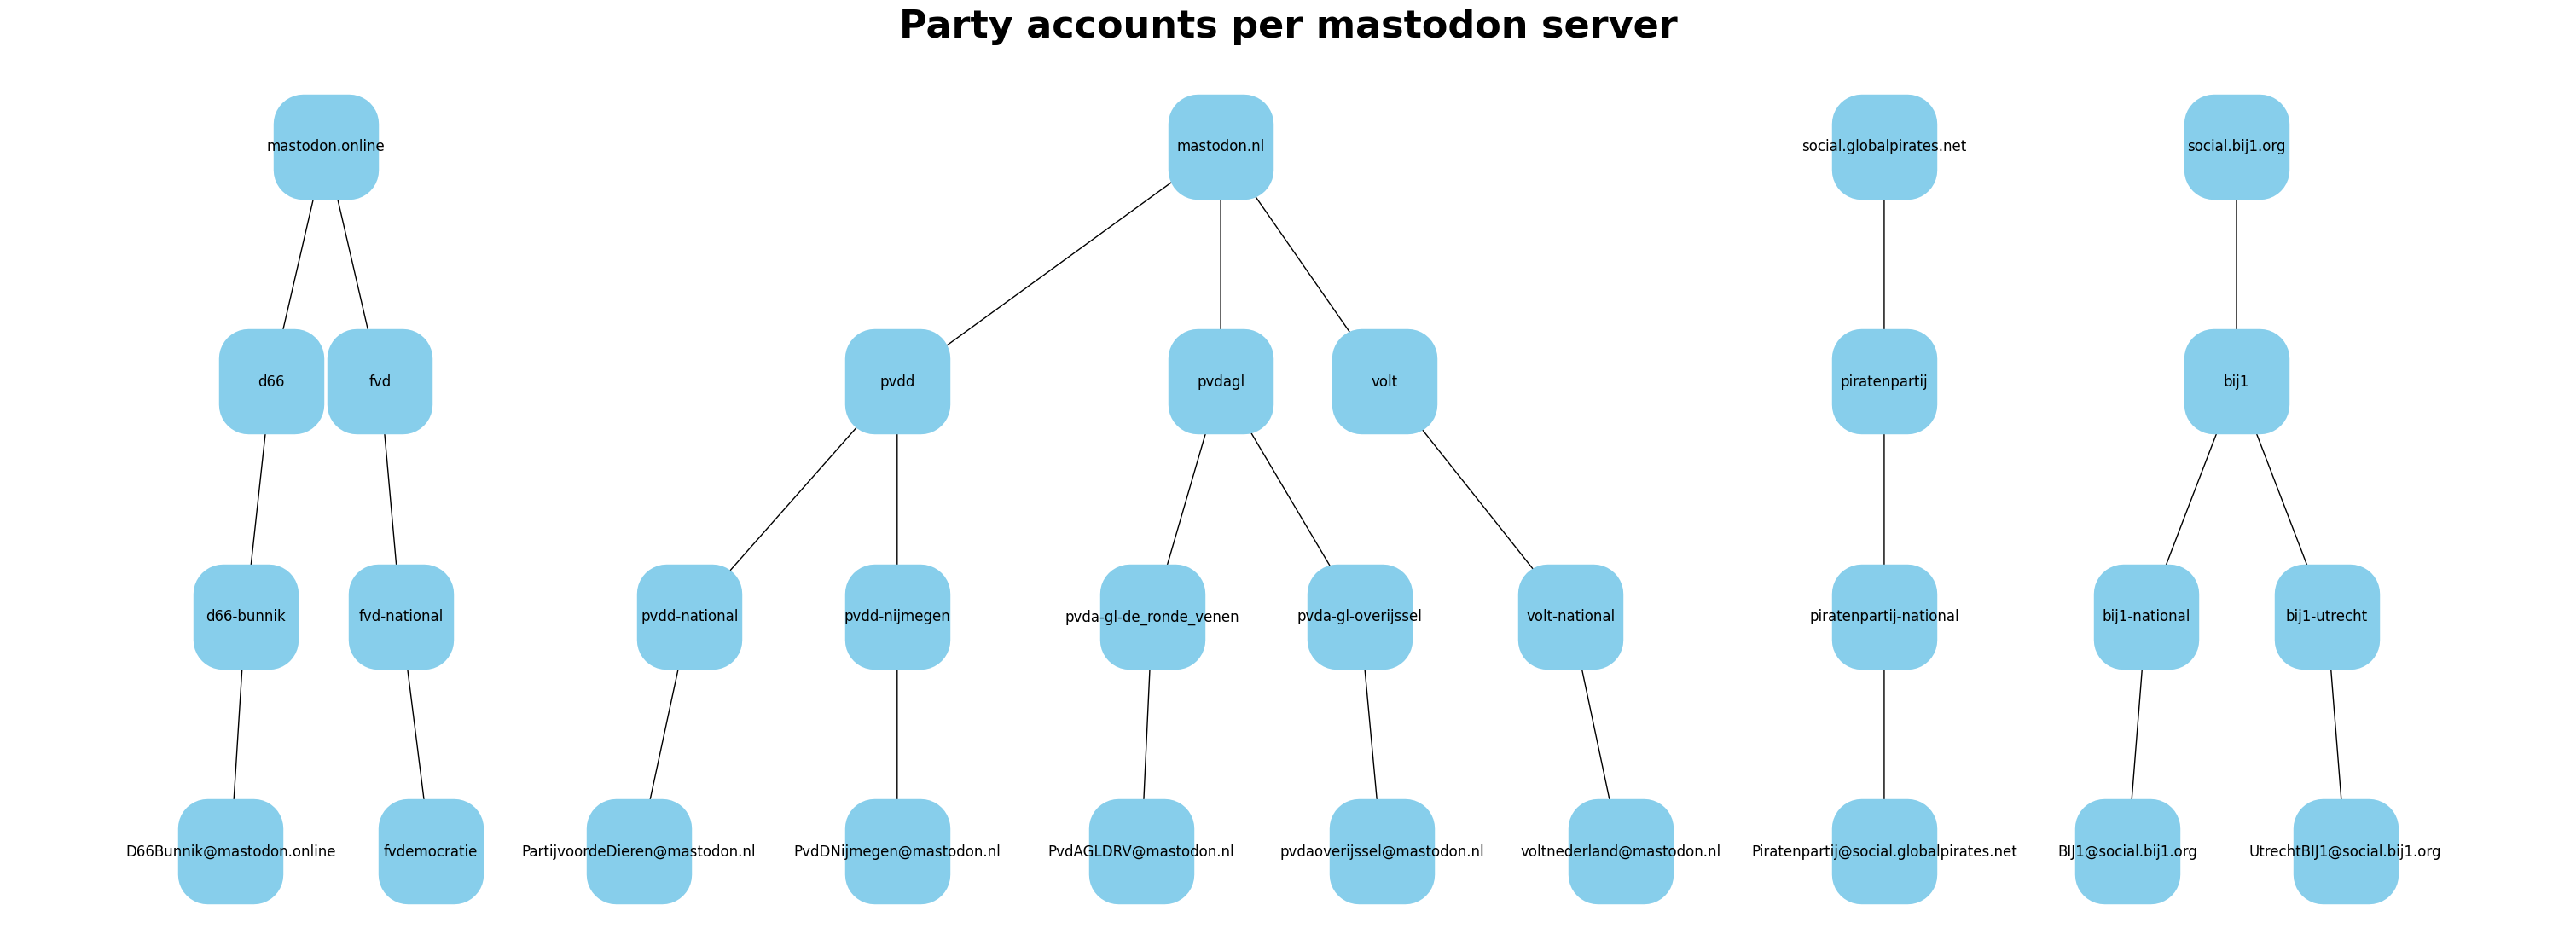
\includegraphics[width=\linewidth]{media/server.png}
  \caption{Tree of party accounts, branching from their respective server}
  \label{fig:servernetwork}
\end{figure}

\begin{figure*}[ht]
  \centering
  \begin{subfigure}[h]{.49\linewidth}
    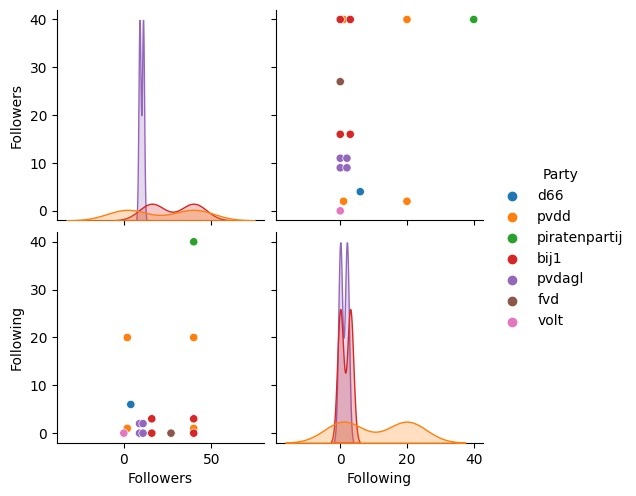
\includegraphics[width=\textwidth]{media/parties-following-counts.jpeg}
    \captionsetup{justification=centering}
    \caption{This is a subcaption}
    \label{fig:partyfollowers}
  \end{subfigure}
  \begin{subfigure}[h]{.49\linewidth}
      \captionsetup{justification=centering}
      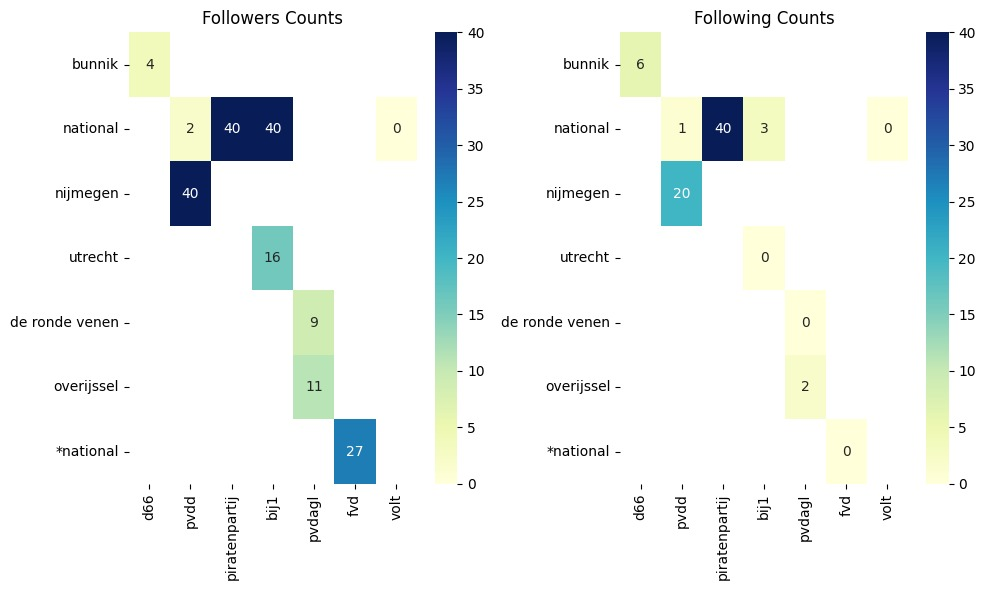
\includegraphics[width=\textwidth]{media/parties-following-region-counts.jpeg}
      \caption{This is a subcaption}
      \label{fig:partyfollowingregions}
  \end{subfigure}
  \caption{Graphs visualizing parties and follower counts}
  \label{fig:partyfollowerstotal}
\end{figure*}


\textbf{Finding M3:} \textit{Out of all parties x parties are present on Mastodon and have instances.}
